\notechapter{N-20221207}{Set Problems, Extremal Counting, and Venn-Diagram Reasoning}

\section{A set construction problem}

The first problem defines a finite set
\[
  A=\{a_1<a_2<\cdots<a_k\}
\]
of positive integers and builds two derived sets, one from sums and one from differences.  The important idea is to use the union \(S\cup T\) without identifying every element exactly, and instead bound its size from below and above.

The sum set contains at least the ordered chain
\[
  2a_1,\ a_1+a_2,\ 2a_2,\ldots,\ a_{k-1}+a_k,\ 2a_k,
\]
so
\[
  |S|\ge2k-1.
\]
The difference set contains
\[
  0,\ a_2-a_1,\ a_3-a_1,\ldots,\ a_k-a_1,
\]
so
\[
  |T|\ge k.
\]
Under the condition of the problem, \(S\cap T=\varnothing\), hence
\[
  |S\cup T|=|S|+|T|\ge3k-1.
\]
On the other hand, all these numbers lie between \(0\) and \(2a_k\), so
\[
  |S\cup T|\le2a_k+1.
\]
Thus
\[
  3k-1\le2a_k+1.
\]
If \(a_k\le2021\), then
\[
  k\le\frac{2\cdot2021+2}{3}=1348.
\]
The construction
\[
  A=\{674,675,\ldots,2021\}
\]
attains this bound, so the maximum is
\[
  |A|=1348.
\]

\section{What this problem teaches}

Using \(S\cup T\) avoids a complicated direct extremal argument.  When a problem asks for the largest possible size of a set, auxiliary sets with structurally forced sizes often reveal the correct bound.

A lower bound comes from a construction.  An upper bound comes from counting constraints.  A complete solution needs both.

\section{A Venn-diagram necessary-and-sufficient problem}

Another problem defines set difference
\[
  A-B=\{x:x\in A,\ x\notin B\}
\]
and asks for the relation among \(A,B,C\) when
\[
  (A-B)\cup(B-A)\subseteq C.
\]
The question asks whether this is equivalent to a condition involving
\[
  A\subseteq(C-B)\cup(B-C)
\]
or
\[
  A\cap B\cap C=\varnothing.
\]

A Venn diagram suggests an algebraic decomposition.  The symmetric difference
\[
  (A-B)\cup(B-A)
\]
is the part where membership in \(A\) and \(B\) differs.  If this is contained in \(C\), then outside \(C\) the sets \(A\) and \(B\) must agree.

The reliable method is to analyze each of the eight Venn regions.  Verbal manipulation alone is unsafe because it can silently merge distinct regions or reverse a complement; region-by-region membership prevents those errors.

\begin{figure}[H]
\centering
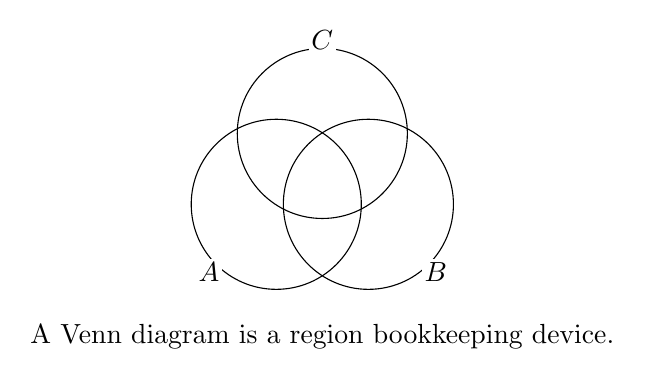
\begin{tikzpicture}[scale=0.9,every node/.style={fill=white,inner sep=1pt}]
  \draw (0,0) circle (1.2);
  \draw (1.3,0) circle (1.2);
  \draw (0.65,1.0) circle (1.2);
  \node at (-0.95,-0.95) {$A$};
  \node at (2.25,-0.95) {$B$};
  \node at (0.65,2.32) {$C$};
  \node[below] at (0.65,-1.65) {A Venn diagram is a region bookkeeping device.};
\end{tikzpicture}
\caption{For three sets one should reason region by region, not by visual guesswork alone.}
\end{figure}

\section{Difference identities}

One useful identity is
\[
  B-C=B\cap C^c.
\]
Therefore
\[
  B-C-(A\cap B)
  =
  B\cap C^c\cap(A\cap B)^c.
\]
Using De Morgan,
\[
  (A\cap B)^c=A^c\cup B^c,
\]
so
\[
  B\cap C^c\cap(A^c\cup B^c)
  =
  (B\cap C^c\cap A^c)\cup(B\cap C^c\cap B^c).
\]
The second term is empty, hence
\[
  B-C-(A\cap B)=B\cap A^c\cap C^c.
\]
This is exactly the kind of algebraic cleanup that a Venn diagram suggests but does not replace.

\section{Coordinate and algebraic exercises}

Algebraic and coordinate exercises involving quadratic expressions, tangent or chord diagrams, and geometric conditions repeatedly use the same pattern:
\begin{enumerate}[(i)]
  \item introduce the unknowns explicitly;
  \item translate each condition into an equation or inequality;
  \item reduce by substitution or by completing the square;
  \item check equality or boundary cases.

\end{enumerate}

Several sketches show lines touching curves or intersecting regions.  Rather than reproducing them as raw images, the important content is the method: a picture tells us which algebraic condition to impose, such as tangency, parallelism, or containment.

\section{A note on proof writing}

A purely diagrammatic method is intuitive but can be unreliable.  Use the diagram to discover the statement, then use set algebra to prove it: geometry finds the path, while formal manipulation makes the path safe.


\section{Extremal set problems: why constructions matter}

In an extremal counting problem, an upper bound is only half the solution; a construction must show sharpness.  For sum sets and difference sets, first prove that the derived sets contain enough elements, then exhibit a set \(A\) attaining the bound.

This is a common combinatorial habit.  Inequalities show impossibility beyond a threshold.  Constructions show that the threshold is real.

\section{Venn diagrams versus proofs}

Venn diagrams are excellent for discovering set identities, but the proof should eventually be written elementwise.  For example,
\[
  A\setminus(B\cup C)=(A\setminus B)\cap(A\setminus C)
\]
is proved by taking an arbitrary \(x\) and translating membership:
\[
  x\in A\setminus(B\cup C)
  \Longleftrightarrow
  x\in A,\ x\notin B,\ x\notin C.
\]
This is exactly the condition for membership in the right-hand side.  The diagram gives intuition; the element chase gives proof.

\section{A wider frame}

Extremal counting and Boolean region decomposition share a common method: replace a vague configuration by a finite list of regions or quantities that can be counted exactly.  The same principle underlies combinatorial proofs, measure decompositions, and sigma-algebra calculations.

\section{Extremal problems: upper bound plus construction}

The sum-set/difference-set problem has the standard shape of extremal combinatorics.  One proves an upper bound by showing that certain auxiliary objects must fit inside a finite container.  Then one gives a construction meeting the bound.

This two-part structure is essential:
\[
  \text{upper bound}+
  \text{matching construction}=\text{exact extremal value}.
\]
A construction alone proves possibility; an upper bound alone proves limitation.  A complete extremal solution needs both.

\section{Additive combinatorics viewpoint}

For a finite set \(A\subseteq\mathbb Z\), the sum set and difference set are
\[
  A+A=\{a+a':a,a'\in A\},\qquad
  A-A=\{a-a':a,a'\in A\}.
\]
The size of these sets measures additive structure.  Arithmetic progressions have unusually small sumsets.  Random sets usually have much larger sumsets.

A central theorem in additive combinatorics is Freiman's philosophy: if \(|A+A|\) is small compared with \(|A|\), then \(A\) must resemble a generalized arithmetic progression.  The elementary problem is a small concrete case of studying what set structure is forced by sum and difference constraints.

\section{Cauchy--Davenport shadow}

In a prime cyclic group \(\mathbb Z/p\mathbb Z\), the Cauchy--Davenport theorem says
\[
  |A+B|\ge \min(p,\ |A|+|B|-1).
\]
This is the modular analogue of the simple lower bound that a sumset of ordered integer sets contains a chain of at least \(|A|+|B|-1\) elements.

The theorem shows that the lower-bound logic in the note is not accidental.  Sumsets are forced to grow unless the ambient group wraps around or the set has special structure.

\section{Boolean atoms and Venn regions}

For three sets \(A,B,C\), the universe is partitioned into at most eight atoms:
\[
  A^{\epsilon_1}\cap B^{\epsilon_2}\cap C^{\epsilon_3},\qquad
  \epsilon_i\in\{0,1\},
\]
where \(A^1=A\) and \(A^0=A^c\).  Every Boolean expression in \(A,B,C\) is a union of some of these atoms.

This gives a systematic proof method: reduce both sides of a set identity to the same atoms.  Venn diagrams are pictures of this atomic decomposition; elementwise proofs are the formal version.

\section{Symmetric difference as addition mod two}

The symmetric difference
\[
  A\triangle B=(A\setminus B)\cup(B\setminus A)
\]
behaves like addition modulo \(2\) on characteristic functions:
\[
  \mathbf 1_{A\triangle B}=\mathbf 1_A+\mathbf 1_B\pmod2.
\]
Thus the power set \(\mathcal P(U)\) becomes a vector space over \(\mathbb F_2\) under symmetric difference.  Intersection acts like multiplication.

This explains why expressions such as \((A-B)\cup(B-A)\) have algebraic structure: they are not just set differences, but mod-two sums of predicates.

\section{Sperner and intersecting-family context}

Many extremal set problems ask for the largest family avoiding a containment or disjointness pattern.  Sperner's theorem says that an antichain \(\mathcal F\subseteq\mathcal P([n])\) satisfies
\[
  |\mathcal F|\le \binom n{\lfloor n/2\rfloor}.
\]
The largest example is the middle layer.

For intersecting families, the Erdős--Ko--Rado theorem says that if \(\mathcal F\subseteq\binom{[n]}k\) is pairwise intersecting and \(n\ge2k\), then
\[
  |\mathcal F|\le\binom{n-1}{k-1}.
\]
The extremal example is a star: all \(k\)-sets containing a fixed element.

These theorems refine the same method: identify the forbidden configuration, prove an upper bound, and classify sharp examples.

\section{Shifting and stability}

Shifting transforms a set family into a more ordered one without changing its size or destroying the relevant forbidden configuration.  Repeated shifting often reduces an extremal problem to a canonical family.

A stability theorem asks more than the maximum: if a family is close to maximum size, must it be structurally close to an extremal example?  This is the research-level continuation of checking equality cases in an elementary inequality.

\section{Extremal sets, Boolean algebra, and stability}

The note combines two important habits.  Extremal counting uses auxiliary sets, upper bounds, and sharp constructions.  Venn reasoning uses Boolean atoms and set algebra.  At a higher level these become additive combinatorics, extremal set theory, vector-space structure over \(\mathbb F_2\), and stability methods.
